% backtracking worksheet template
\documentclass[leqno, 12pt]{article}
\usepackage{tikz}  
\usetikzlibrary{positioning}
\usetikzlibrary {arrows.meta}
\usepackage[a4paper, portrait, margin=1cm]{geometry}
\usepackage{multicol}
\usepackage{fancyhdr}

\tikzset{backtrack/.style={rectangle,draw=black,fill=white,
inner sep=2pt,minimum height=32pt, minimum width=20mm}}
\tikzset{backtrackeq/.style={rectangle,draw=black,fill=white,
inner sep=2pt,minimum height=12pt, minimum width=20mm}}
\tikzset{backtrackstep/.style={rectangle,draw=none,fill=white,
inner sep=2pt,minimum height=12pt, minimum width=20mm}}

\def \HeadingAnswers {\section*{\Huge Name: \underline{\hspace{8cm}} \hfill Date: \underline{\hspace{3cm}}}
{1-step backtracking: Answers} \vspace{1pt}\hrule}

% raise footer with page number; no header
\fancypagestyle{myfancypagestyle}{
  \fancyhf{}% clear all header and footer fields
  \renewcommand{\headrulewidth}{0pt} % no rule under header
  \fancyfoot[C] {\thepage} \setlength{\footskip}{6pt} % raise page number 6pt
}
\pagestyle{myfancypagestyle}  % apply myfancypagestyle

\begin{document}
    \HeadingAnswers
    \vspace{-5mm}
    \begin{multicols}{2}
        \begin{equation}
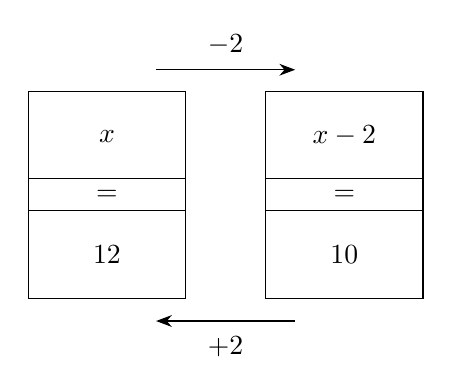
\begin{tikzpicture}[baseline={([yshift=-1pt]current bounding box.north)}]

    \node[backtrack] (boxA) at (0, 0) {$x$};
    \node[backtrack] (boxB) [right=1cm of boxA] {$x-2$};
 
    \node[backtrackeq] (boxAeq) [below=-1pt of boxA] {$=$};
    \node[backtrackeq] (boxBeq) [below=-1pt of boxB] {$=$};

    \node[backtrack] (boxArev) [below=-1pt of boxAeq] {$12$};
    \node[backtrack] (boxBrev) [below=-1pt of boxBeq] {$10$};

    \node(boxAr) at ([yshift=24pt,xshift=5mm]boxA) { };
    \node(boxBl) at ([yshift=24pt,xshift=-5mm]boxB) { };
    \draw [line width=0.4pt,-{Stealth[length=2mm]}] (boxAr)  --node[backtrackstep, above=3.0pt] {$-2$} (boxBl);
    
    \node(boxBrevl) at ([yshift=-24pt,xshift=-5mm]boxBrev) { };
    \node(boxArevr) at ([yshift=-24pt,xshift=5mm]boxArev) { };
    \draw [line width=0.4pt,-{Stealth[length=2mm]}] (boxBrevl)  --node[backtrackstep, below=3.0pt] {$+2$} (boxArevr);

\end{tikzpicture}
\end{equation}


\vspace{-2pt}\begin{equation}
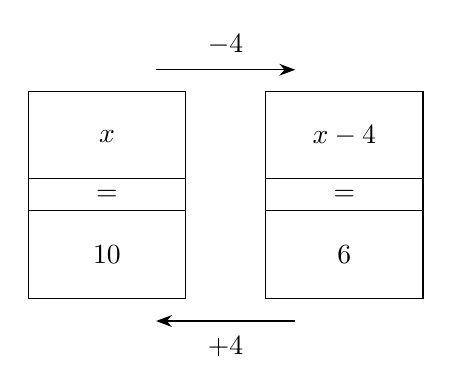
\begin{tikzpicture}[baseline={([yshift=-1pt]current bounding box.north)}]

    \node[backtrack] (boxA) at (0, 0) {$x$};
    \node[backtrack] (boxB) [right=1cm of boxA] {$x-4$};
 
    \node[backtrackeq] (boxAeq) [below=-1pt of boxA] {$=$};
    \node[backtrackeq] (boxBeq) [below=-1pt of boxB] {$=$};

    \node[backtrack] (boxArev) [below=-1pt of boxAeq] {$10$};
    \node[backtrack] (boxBrev) [below=-1pt of boxBeq] {$6$};

    \node(boxAr) at ([yshift=24pt,xshift=5mm]boxA) { };
    \node(boxBl) at ([yshift=24pt,xshift=-5mm]boxB) { };
    \draw [line width=0.4pt,-{Stealth[length=2mm]}] (boxAr)  --node[backtrackstep, above=3.0pt] {$-4$} (boxBl);
    
    \node(boxBrevl) at ([yshift=-24pt,xshift=-5mm]boxBrev) { };
    \node(boxArevr) at ([yshift=-24pt,xshift=5mm]boxArev) { };
    \draw [line width=0.4pt,-{Stealth[length=2mm]}] (boxBrevl)  --node[backtrackstep, below=3.0pt] {$+4$} (boxArevr);

\end{tikzpicture}
\end{equation}


\vspace{-2pt}\begin{equation}
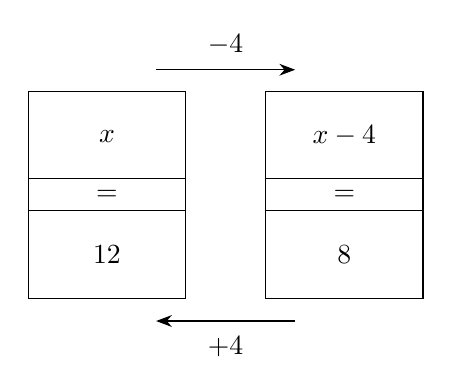
\begin{tikzpicture}[baseline={([yshift=-1pt]current bounding box.north)}]

    \node[backtrack] (boxA) at (0, 0) {$x$};
    \node[backtrack] (boxB) [right=1cm of boxA] {$x-4$};
 
    \node[backtrackeq] (boxAeq) [below=-1pt of boxA] {$=$};
    \node[backtrackeq] (boxBeq) [below=-1pt of boxB] {$=$};

    \node[backtrack] (boxArev) [below=-1pt of boxAeq] {$12$};
    \node[backtrack] (boxBrev) [below=-1pt of boxBeq] {$8$};

    \node(boxAr) at ([yshift=24pt,xshift=5mm]boxA) { };
    \node(boxBl) at ([yshift=24pt,xshift=-5mm]boxB) { };
    \draw [line width=0.4pt,-{Stealth[length=2mm]}] (boxAr)  --node[backtrackstep, above=3.0pt] {$-4$} (boxBl);
    
    \node(boxBrevl) at ([yshift=-24pt,xshift=-5mm]boxBrev) { };
    \node(boxArevr) at ([yshift=-24pt,xshift=5mm]boxArev) { };
    \draw [line width=0.4pt,-{Stealth[length=2mm]}] (boxBrevl)  --node[backtrackstep, below=3.0pt] {$+4$} (boxArevr);

\end{tikzpicture}
\end{equation}


\vspace{-2pt}\begin{equation}
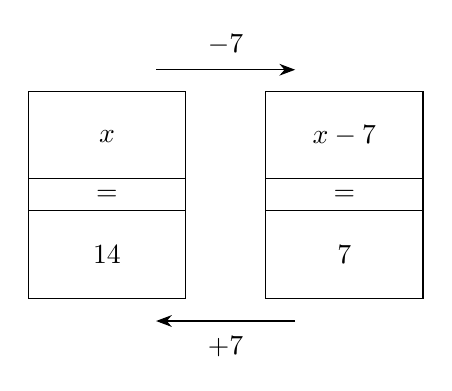
\begin{tikzpicture}[baseline={([yshift=-1pt]current bounding box.north)}]

    \node[backtrack] (boxA) at (0, 0) {$x$};
    \node[backtrack] (boxB) [right=1cm of boxA] {$x-7$};
 
    \node[backtrackeq] (boxAeq) [below=-1pt of boxA] {$=$};
    \node[backtrackeq] (boxBeq) [below=-1pt of boxB] {$=$};

    \node[backtrack] (boxArev) [below=-1pt of boxAeq] {$14$};
    \node[backtrack] (boxBrev) [below=-1pt of boxBeq] {$7$};

    \node(boxAr) at ([yshift=24pt,xshift=5mm]boxA) { };
    \node(boxBl) at ([yshift=24pt,xshift=-5mm]boxB) { };
    \draw [line width=0.4pt,-{Stealth[length=2mm]}] (boxAr)  --node[backtrackstep, above=3.0pt] {$-7$} (boxBl);
    
    \node(boxBrevl) at ([yshift=-24pt,xshift=-5mm]boxBrev) { };
    \node(boxArevr) at ([yshift=-24pt,xshift=5mm]boxArev) { };
    \draw [line width=0.4pt,-{Stealth[length=2mm]}] (boxBrevl)  --node[backtrackstep, below=3.0pt] {$+7$} (boxArevr);

\end{tikzpicture}
\end{equation}


\vspace{-2pt}\begin{equation}
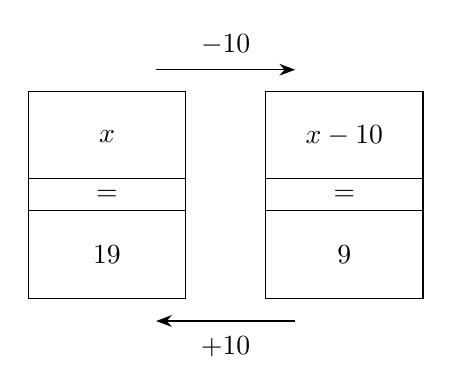
\begin{tikzpicture}[baseline={([yshift=-1pt]current bounding box.north)}]

    \node[backtrack] (boxA) at (0, 0) {$x$};
    \node[backtrack] (boxB) [right=1cm of boxA] {$x-10$};
 
    \node[backtrackeq] (boxAeq) [below=-1pt of boxA] {$=$};
    \node[backtrackeq] (boxBeq) [below=-1pt of boxB] {$=$};

    \node[backtrack] (boxArev) [below=-1pt of boxAeq] {$19$};
    \node[backtrack] (boxBrev) [below=-1pt of boxBeq] {$9$};

    \node(boxAr) at ([yshift=24pt,xshift=5mm]boxA) { };
    \node(boxBl) at ([yshift=24pt,xshift=-5mm]boxB) { };
    \draw [line width=0.4pt,-{Stealth[length=2mm]}] (boxAr)  --node[backtrackstep, above=3.0pt] {$-10$} (boxBl);
    
    \node(boxBrevl) at ([yshift=-24pt,xshift=-5mm]boxBrev) { };
    \node(boxArevr) at ([yshift=-24pt,xshift=5mm]boxArev) { };
    \draw [line width=0.4pt,-{Stealth[length=2mm]}] (boxBrevl)  --node[backtrackstep, below=3.0pt] {$+10$} (boxArevr);

\end{tikzpicture}
\end{equation}


\vspace{-2pt}\begin{equation}
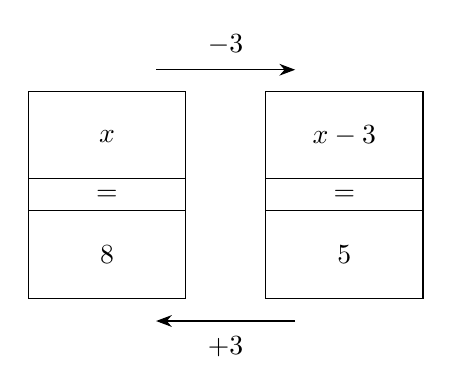
\begin{tikzpicture}[baseline={([yshift=-1pt]current bounding box.north)}]

    \node[backtrack] (boxA) at (0, 0) {$x$};
    \node[backtrack] (boxB) [right=1cm of boxA] {$x-3$};
 
    \node[backtrackeq] (boxAeq) [below=-1pt of boxA] {$=$};
    \node[backtrackeq] (boxBeq) [below=-1pt of boxB] {$=$};

    \node[backtrack] (boxArev) [below=-1pt of boxAeq] {$8$};
    \node[backtrack] (boxBrev) [below=-1pt of boxBeq] {$5$};

    \node(boxAr) at ([yshift=24pt,xshift=5mm]boxA) { };
    \node(boxBl) at ([yshift=24pt,xshift=-5mm]boxB) { };
    \draw [line width=0.4pt,-{Stealth[length=2mm]}] (boxAr)  --node[backtrackstep, above=3.0pt] {$-3$} (boxBl);
    
    \node(boxBrevl) at ([yshift=-24pt,xshift=-5mm]boxBrev) { };
    \node(boxArevr) at ([yshift=-24pt,xshift=5mm]boxArev) { };
    \draw [line width=0.4pt,-{Stealth[length=2mm]}] (boxBrevl)  --node[backtrackstep, below=3.0pt] {$+3$} (boxArevr);

\end{tikzpicture}
\end{equation}


\vspace{-2pt}\begin{equation}
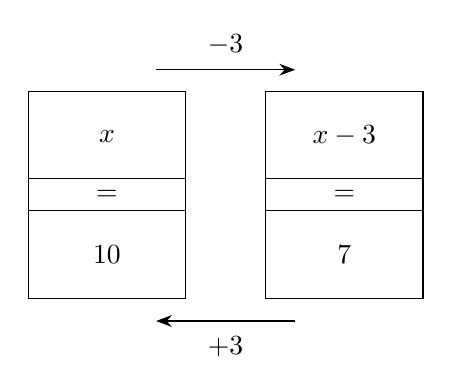
\begin{tikzpicture}[baseline={([yshift=-1pt]current bounding box.north)}]

    \node[backtrack] (boxA) at (0, 0) {$x$};
    \node[backtrack] (boxB) [right=1cm of boxA] {$x-3$};
 
    \node[backtrackeq] (boxAeq) [below=-1pt of boxA] {$=$};
    \node[backtrackeq] (boxBeq) [below=-1pt of boxB] {$=$};

    \node[backtrack] (boxArev) [below=-1pt of boxAeq] {$10$};
    \node[backtrack] (boxBrev) [below=-1pt of boxBeq] {$7$};

    \node(boxAr) at ([yshift=24pt,xshift=5mm]boxA) { };
    \node(boxBl) at ([yshift=24pt,xshift=-5mm]boxB) { };
    \draw [line width=0.4pt,-{Stealth[length=2mm]}] (boxAr)  --node[backtrackstep, above=3.0pt] {$-3$} (boxBl);
    
    \node(boxBrevl) at ([yshift=-24pt,xshift=-5mm]boxBrev) { };
    \node(boxArevr) at ([yshift=-24pt,xshift=5mm]boxArev) { };
    \draw [line width=0.4pt,-{Stealth[length=2mm]}] (boxBrevl)  --node[backtrackstep, below=3.0pt] {$+3$} (boxArevr);

\end{tikzpicture}
\end{equation}


\vspace{-2pt}\begin{equation}
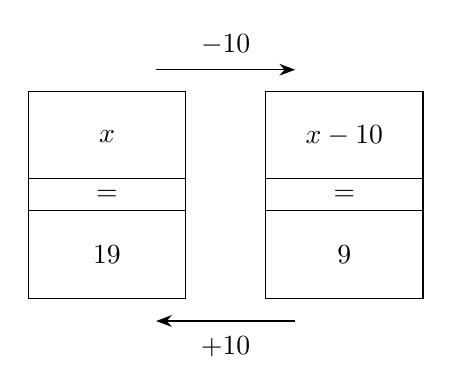
\begin{tikzpicture}[baseline={([yshift=-1pt]current bounding box.north)}]

    \node[backtrack] (boxA) at (0, 0) {$x$};
    \node[backtrack] (boxB) [right=1cm of boxA] {$x-10$};
 
    \node[backtrackeq] (boxAeq) [below=-1pt of boxA] {$=$};
    \node[backtrackeq] (boxBeq) [below=-1pt of boxB] {$=$};

    \node[backtrack] (boxArev) [below=-1pt of boxAeq] {$19$};
    \node[backtrack] (boxBrev) [below=-1pt of boxBeq] {$9$};

    \node(boxAr) at ([yshift=24pt,xshift=5mm]boxA) { };
    \node(boxBl) at ([yshift=24pt,xshift=-5mm]boxB) { };
    \draw [line width=0.4pt,-{Stealth[length=2mm]}] (boxAr)  --node[backtrackstep, above=3.0pt] {$-10$} (boxBl);
    
    \node(boxBrevl) at ([yshift=-24pt,xshift=-5mm]boxBrev) { };
    \node(boxArevr) at ([yshift=-24pt,xshift=5mm]boxArev) { };
    \draw [line width=0.4pt,-{Stealth[length=2mm]}] (boxBrevl)  --node[backtrackstep, below=3.0pt] {$+10$} (boxArevr);

\end{tikzpicture}
\end{equation}


\vspace{-2pt}\begin{equation}
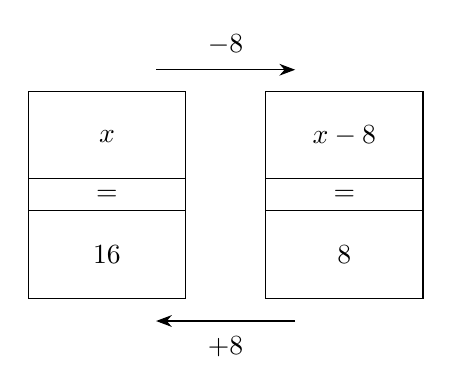
\begin{tikzpicture}[baseline={([yshift=-1pt]current bounding box.north)}]

    \node[backtrack] (boxA) at (0, 0) {$x$};
    \node[backtrack] (boxB) [right=1cm of boxA] {$x-8$};
 
    \node[backtrackeq] (boxAeq) [below=-1pt of boxA] {$=$};
    \node[backtrackeq] (boxBeq) [below=-1pt of boxB] {$=$};

    \node[backtrack] (boxArev) [below=-1pt of boxAeq] {$16$};
    \node[backtrack] (boxBrev) [below=-1pt of boxBeq] {$8$};

    \node(boxAr) at ([yshift=24pt,xshift=5mm]boxA) { };
    \node(boxBl) at ([yshift=24pt,xshift=-5mm]boxB) { };
    \draw [line width=0.4pt,-{Stealth[length=2mm]}] (boxAr)  --node[backtrackstep, above=3.0pt] {$-8$} (boxBl);
    
    \node(boxBrevl) at ([yshift=-24pt,xshift=-5mm]boxBrev) { };
    \node(boxArevr) at ([yshift=-24pt,xshift=5mm]boxArev) { };
    \draw [line width=0.4pt,-{Stealth[length=2mm]}] (boxBrevl)  --node[backtrackstep, below=3.0pt] {$+8$} (boxArevr);

\end{tikzpicture}
\end{equation}


\vspace{-2pt}\begin{equation}
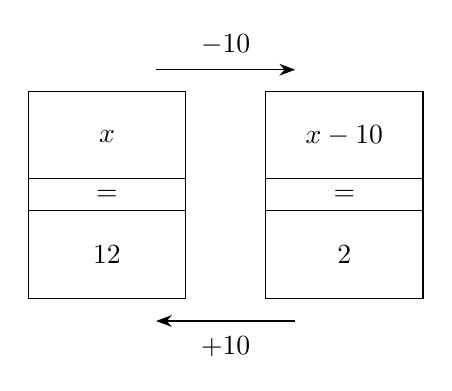
\begin{tikzpicture}[baseline={([yshift=-1pt]current bounding box.north)}]

    \node[backtrack] (boxA) at (0, 0) {$x$};
    \node[backtrack] (boxB) [right=1cm of boxA] {$x-10$};
 
    \node[backtrackeq] (boxAeq) [below=-1pt of boxA] {$=$};
    \node[backtrackeq] (boxBeq) [below=-1pt of boxB] {$=$};

    \node[backtrack] (boxArev) [below=-1pt of boxAeq] {$12$};
    \node[backtrack] (boxBrev) [below=-1pt of boxBeq] {$2$};

    \node(boxAr) at ([yshift=24pt,xshift=5mm]boxA) { };
    \node(boxBl) at ([yshift=24pt,xshift=-5mm]boxB) { };
    \draw [line width=0.4pt,-{Stealth[length=2mm]}] (boxAr)  --node[backtrackstep, above=3.0pt] {$-10$} (boxBl);
    
    \node(boxBrevl) at ([yshift=-24pt,xshift=-5mm]boxBrev) { };
    \node(boxArevr) at ([yshift=-24pt,xshift=5mm]boxArev) { };
    \draw [line width=0.4pt,-{Stealth[length=2mm]}] (boxBrevl)  --node[backtrackstep, below=3.0pt] {$+10$} (boxArevr);

\end{tikzpicture}
\end{equation}


\vspace{-2pt}\begin{equation}
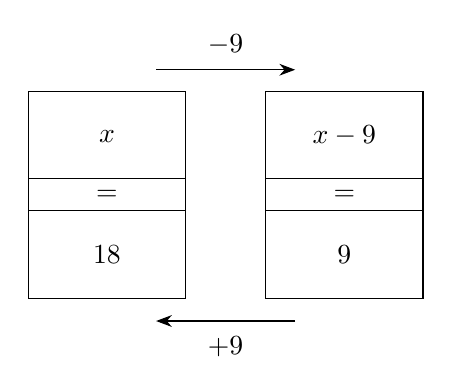
\begin{tikzpicture}[baseline={([yshift=-1pt]current bounding box.north)}]

    \node[backtrack] (boxA) at (0, 0) {$x$};
    \node[backtrack] (boxB) [right=1cm of boxA] {$x-9$};
 
    \node[backtrackeq] (boxAeq) [below=-1pt of boxA] {$=$};
    \node[backtrackeq] (boxBeq) [below=-1pt of boxB] {$=$};

    \node[backtrack] (boxArev) [below=-1pt of boxAeq] {$18$};
    \node[backtrack] (boxBrev) [below=-1pt of boxBeq] {$9$};

    \node(boxAr) at ([yshift=24pt,xshift=5mm]boxA) { };
    \node(boxBl) at ([yshift=24pt,xshift=-5mm]boxB) { };
    \draw [line width=0.4pt,-{Stealth[length=2mm]}] (boxAr)  --node[backtrackstep, above=3.0pt] {$-9$} (boxBl);
    
    \node(boxBrevl) at ([yshift=-24pt,xshift=-5mm]boxBrev) { };
    \node(boxArevr) at ([yshift=-24pt,xshift=5mm]boxArev) { };
    \draw [line width=0.4pt,-{Stealth[length=2mm]}] (boxBrevl)  --node[backtrackstep, below=3.0pt] {$+9$} (boxArevr);

\end{tikzpicture}
\end{equation}


\vspace{-2pt}\begin{equation}
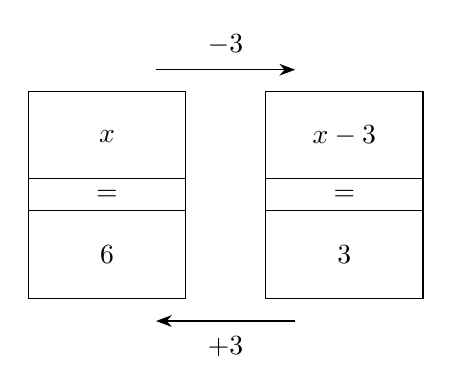
\begin{tikzpicture}[baseline={([yshift=-1pt]current bounding box.north)}]

    \node[backtrack] (boxA) at (0, 0) {$x$};
    \node[backtrack] (boxB) [right=1cm of boxA] {$x-3$};
 
    \node[backtrackeq] (boxAeq) [below=-1pt of boxA] {$=$};
    \node[backtrackeq] (boxBeq) [below=-1pt of boxB] {$=$};

    \node[backtrack] (boxArev) [below=-1pt of boxAeq] {$6$};
    \node[backtrack] (boxBrev) [below=-1pt of boxBeq] {$3$};

    \node(boxAr) at ([yshift=24pt,xshift=5mm]boxA) { };
    \node(boxBl) at ([yshift=24pt,xshift=-5mm]boxB) { };
    \draw [line width=0.4pt,-{Stealth[length=2mm]}] (boxAr)  --node[backtrackstep, above=3.0pt] {$-3$} (boxBl);
    
    \node(boxBrevl) at ([yshift=-24pt,xshift=-5mm]boxBrev) { };
    \node(boxArevr) at ([yshift=-24pt,xshift=5mm]boxArev) { };
    \draw [line width=0.4pt,-{Stealth[length=2mm]}] (boxBrevl)  --node[backtrackstep, below=3.0pt] {$+3$} (boxArevr);

\end{tikzpicture}
\end{equation}


\vspace{-2pt}\begin{equation}
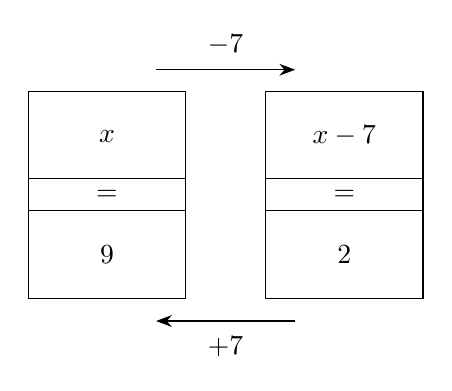
\begin{tikzpicture}[baseline={([yshift=-1pt]current bounding box.north)}]

    \node[backtrack] (boxA) at (0, 0) {$x$};
    \node[backtrack] (boxB) [right=1cm of boxA] {$x-7$};
 
    \node[backtrackeq] (boxAeq) [below=-1pt of boxA] {$=$};
    \node[backtrackeq] (boxBeq) [below=-1pt of boxB] {$=$};

    \node[backtrack] (boxArev) [below=-1pt of boxAeq] {$9$};
    \node[backtrack] (boxBrev) [below=-1pt of boxBeq] {$2$};

    \node(boxAr) at ([yshift=24pt,xshift=5mm]boxA) { };
    \node(boxBl) at ([yshift=24pt,xshift=-5mm]boxB) { };
    \draw [line width=0.4pt,-{Stealth[length=2mm]}] (boxAr)  --node[backtrackstep, above=3.0pt] {$-7$} (boxBl);
    
    \node(boxBrevl) at ([yshift=-24pt,xshift=-5mm]boxBrev) { };
    \node(boxArevr) at ([yshift=-24pt,xshift=5mm]boxArev) { };
    \draw [line width=0.4pt,-{Stealth[length=2mm]}] (boxBrevl)  --node[backtrackstep, below=3.0pt] {$+7$} (boxArevr);

\end{tikzpicture}
\end{equation}


\vspace{-2pt}\begin{equation}
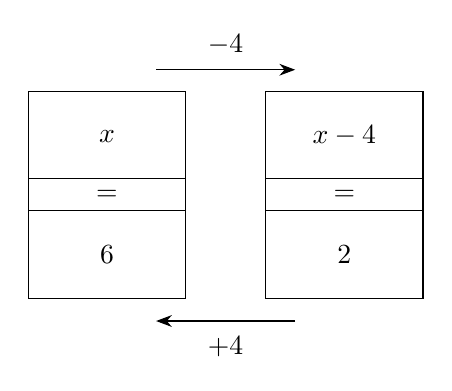
\begin{tikzpicture}[baseline={([yshift=-1pt]current bounding box.north)}]

    \node[backtrack] (boxA) at (0, 0) {$x$};
    \node[backtrack] (boxB) [right=1cm of boxA] {$x-4$};
 
    \node[backtrackeq] (boxAeq) [below=-1pt of boxA] {$=$};
    \node[backtrackeq] (boxBeq) [below=-1pt of boxB] {$=$};

    \node[backtrack] (boxArev) [below=-1pt of boxAeq] {$6$};
    \node[backtrack] (boxBrev) [below=-1pt of boxBeq] {$2$};

    \node(boxAr) at ([yshift=24pt,xshift=5mm]boxA) { };
    \node(boxBl) at ([yshift=24pt,xshift=-5mm]boxB) { };
    \draw [line width=0.4pt,-{Stealth[length=2mm]}] (boxAr)  --node[backtrackstep, above=3.0pt] {$-4$} (boxBl);
    
    \node(boxBrevl) at ([yshift=-24pt,xshift=-5mm]boxBrev) { };
    \node(boxArevr) at ([yshift=-24pt,xshift=5mm]boxArev) { };
    \draw [line width=0.4pt,-{Stealth[length=2mm]}] (boxBrevl)  --node[backtrackstep, below=3.0pt] {$+4$} (boxArevr);

\end{tikzpicture}
\end{equation}


\vspace{-2pt}\begin{equation}
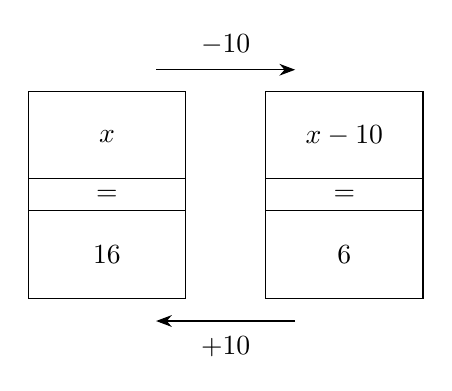
\begin{tikzpicture}[baseline={([yshift=-1pt]current bounding box.north)}]

    \node[backtrack] (boxA) at (0, 0) {$x$};
    \node[backtrack] (boxB) [right=1cm of boxA] {$x-10$};
 
    \node[backtrackeq] (boxAeq) [below=-1pt of boxA] {$=$};
    \node[backtrackeq] (boxBeq) [below=-1pt of boxB] {$=$};

    \node[backtrack] (boxArev) [below=-1pt of boxAeq] {$16$};
    \node[backtrack] (boxBrev) [below=-1pt of boxBeq] {$6$};

    \node(boxAr) at ([yshift=24pt,xshift=5mm]boxA) { };
    \node(boxBl) at ([yshift=24pt,xshift=-5mm]boxB) { };
    \draw [line width=0.4pt,-{Stealth[length=2mm]}] (boxAr)  --node[backtrackstep, above=3.0pt] {$-10$} (boxBl);
    
    \node(boxBrevl) at ([yshift=-24pt,xshift=-5mm]boxBrev) { };
    \node(boxArevr) at ([yshift=-24pt,xshift=5mm]boxArev) { };
    \draw [line width=0.4pt,-{Stealth[length=2mm]}] (boxBrevl)  --node[backtrackstep, below=3.0pt] {$+10$} (boxArevr);

\end{tikzpicture}
\end{equation}


\vspace{-2pt}\begin{equation}
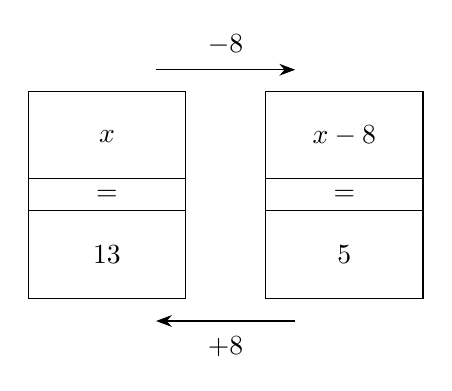
\begin{tikzpicture}[baseline={([yshift=-1pt]current bounding box.north)}]

    \node[backtrack] (boxA) at (0, 0) {$x$};
    \node[backtrack] (boxB) [right=1cm of boxA] {$x-8$};
 
    \node[backtrackeq] (boxAeq) [below=-1pt of boxA] {$=$};
    \node[backtrackeq] (boxBeq) [below=-1pt of boxB] {$=$};

    \node[backtrack] (boxArev) [below=-1pt of boxAeq] {$13$};
    \node[backtrack] (boxBrev) [below=-1pt of boxBeq] {$5$};

    \node(boxAr) at ([yshift=24pt,xshift=5mm]boxA) { };
    \node(boxBl) at ([yshift=24pt,xshift=-5mm]boxB) { };
    \draw [line width=0.4pt,-{Stealth[length=2mm]}] (boxAr)  --node[backtrackstep, above=3.0pt] {$-8$} (boxBl);
    
    \node(boxBrevl) at ([yshift=-24pt,xshift=-5mm]boxBrev) { };
    \node(boxArevr) at ([yshift=-24pt,xshift=5mm]boxArev) { };
    \draw [line width=0.4pt,-{Stealth[length=2mm]}] (boxBrevl)  --node[backtrackstep, below=3.0pt] {$+8$} (boxArevr);

\end{tikzpicture}
\end{equation}


\vspace{-2pt}\begin{equation}
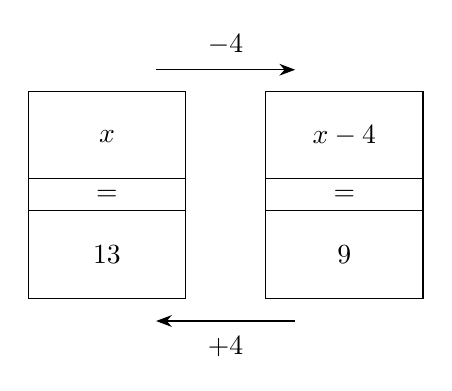
\begin{tikzpicture}[baseline={([yshift=-1pt]current bounding box.north)}]

    \node[backtrack] (boxA) at (0, 0) {$x$};
    \node[backtrack] (boxB) [right=1cm of boxA] {$x-4$};
 
    \node[backtrackeq] (boxAeq) [below=-1pt of boxA] {$=$};
    \node[backtrackeq] (boxBeq) [below=-1pt of boxB] {$=$};

    \node[backtrack] (boxArev) [below=-1pt of boxAeq] {$13$};
    \node[backtrack] (boxBrev) [below=-1pt of boxBeq] {$9$};

    \node(boxAr) at ([yshift=24pt,xshift=5mm]boxA) { };
    \node(boxBl) at ([yshift=24pt,xshift=-5mm]boxB) { };
    \draw [line width=0.4pt,-{Stealth[length=2mm]}] (boxAr)  --node[backtrackstep, above=3.0pt] {$-4$} (boxBl);
    
    \node(boxBrevl) at ([yshift=-24pt,xshift=-5mm]boxBrev) { };
    \node(boxArevr) at ([yshift=-24pt,xshift=5mm]boxArev) { };
    \draw [line width=0.4pt,-{Stealth[length=2mm]}] (boxBrevl)  --node[backtrackstep, below=3.0pt] {$+4$} (boxArevr);

\end{tikzpicture}
\end{equation}


\vspace{-2pt}\begin{equation}
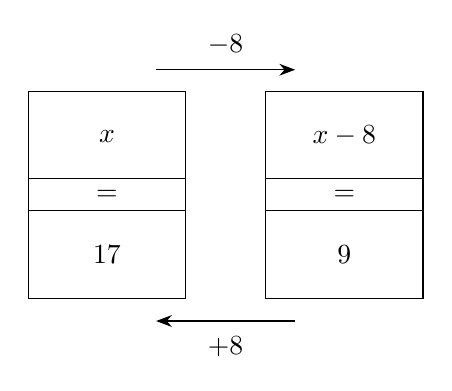
\begin{tikzpicture}[baseline={([yshift=-1pt]current bounding box.north)}]

    \node[backtrack] (boxA) at (0, 0) {$x$};
    \node[backtrack] (boxB) [right=1cm of boxA] {$x-8$};
 
    \node[backtrackeq] (boxAeq) [below=-1pt of boxA] {$=$};
    \node[backtrackeq] (boxBeq) [below=-1pt of boxB] {$=$};

    \node[backtrack] (boxArev) [below=-1pt of boxAeq] {$17$};
    \node[backtrack] (boxBrev) [below=-1pt of boxBeq] {$9$};

    \node(boxAr) at ([yshift=24pt,xshift=5mm]boxA) { };
    \node(boxBl) at ([yshift=24pt,xshift=-5mm]boxB) { };
    \draw [line width=0.4pt,-{Stealth[length=2mm]}] (boxAr)  --node[backtrackstep, above=3.0pt] {$-8$} (boxBl);
    
    \node(boxBrevl) at ([yshift=-24pt,xshift=-5mm]boxBrev) { };
    \node(boxArevr) at ([yshift=-24pt,xshift=5mm]boxArev) { };
    \draw [line width=0.4pt,-{Stealth[length=2mm]}] (boxBrevl)  --node[backtrackstep, below=3.0pt] {$+8$} (boxArevr);

\end{tikzpicture}
\end{equation}


\vspace{-2pt}\begin{equation}
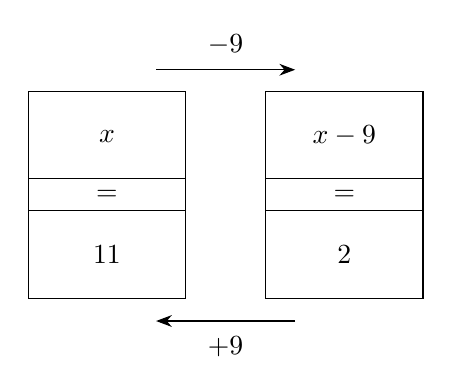
\begin{tikzpicture}[baseline={([yshift=-1pt]current bounding box.north)}]

    \node[backtrack] (boxA) at (0, 0) {$x$};
    \node[backtrack] (boxB) [right=1cm of boxA] {$x-9$};
 
    \node[backtrackeq] (boxAeq) [below=-1pt of boxA] {$=$};
    \node[backtrackeq] (boxBeq) [below=-1pt of boxB] {$=$};

    \node[backtrack] (boxArev) [below=-1pt of boxAeq] {$11$};
    \node[backtrack] (boxBrev) [below=-1pt of boxBeq] {$2$};

    \node(boxAr) at ([yshift=24pt,xshift=5mm]boxA) { };
    \node(boxBl) at ([yshift=24pt,xshift=-5mm]boxB) { };
    \draw [line width=0.4pt,-{Stealth[length=2mm]}] (boxAr)  --node[backtrackstep, above=3.0pt] {$-9$} (boxBl);
    
    \node(boxBrevl) at ([yshift=-24pt,xshift=-5mm]boxBrev) { };
    \node(boxArevr) at ([yshift=-24pt,xshift=5mm]boxArev) { };
    \draw [line width=0.4pt,-{Stealth[length=2mm]}] (boxBrevl)  --node[backtrackstep, below=3.0pt] {$+9$} (boxArevr);

\end{tikzpicture}
\end{equation}


\vspace{-2pt}\begin{equation}
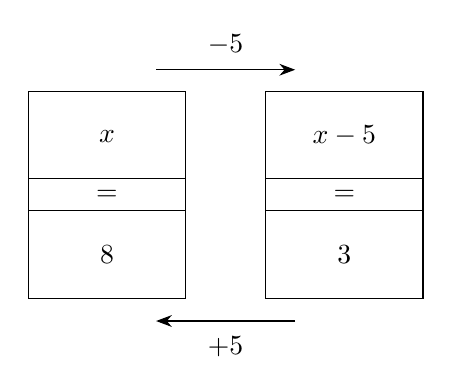
\begin{tikzpicture}[baseline={([yshift=-1pt]current bounding box.north)}]

    \node[backtrack] (boxA) at (0, 0) {$x$};
    \node[backtrack] (boxB) [right=1cm of boxA] {$x-5$};
 
    \node[backtrackeq] (boxAeq) [below=-1pt of boxA] {$=$};
    \node[backtrackeq] (boxBeq) [below=-1pt of boxB] {$=$};

    \node[backtrack] (boxArev) [below=-1pt of boxAeq] {$8$};
    \node[backtrack] (boxBrev) [below=-1pt of boxBeq] {$3$};

    \node(boxAr) at ([yshift=24pt,xshift=5mm]boxA) { };
    \node(boxBl) at ([yshift=24pt,xshift=-5mm]boxB) { };
    \draw [line width=0.4pt,-{Stealth[length=2mm]}] (boxAr)  --node[backtrackstep, above=3.0pt] {$-5$} (boxBl);
    
    \node(boxBrevl) at ([yshift=-24pt,xshift=-5mm]boxBrev) { };
    \node(boxArevr) at ([yshift=-24pt,xshift=5mm]boxArev) { };
    \draw [line width=0.4pt,-{Stealth[length=2mm]}] (boxBrevl)  --node[backtrackstep, below=3.0pt] {$+5$} (boxArevr);

\end{tikzpicture}
\end{equation}


\vspace{-2pt}
    \end{multicols}
\end{document}
